\documentclass{beamer}
\usepackage{verbatim}

\mode<presentation>
{
  \usetheme{default}
  \usecolortheme{default}
  \usefonttheme{default}
  \setbeamertemplate{navigation symbols}{}
  \setbeamertemplate{caption}[numbered]
} 
\usepackage{caption}
\usepackage[english]{babel}
\usepackage[utf8x]{inputenc}

\title[Your Short Title]{Magneto-static Analysis of a Brushless DC Motor}
\author{\small Tom Ginsberg, Brendan Posehn}
\date{}

\begin{document}

\begin{frame}
    \vspace{0.5cm}
  \titlepage
    \vspace{-1.5cm}
  \begin{center}
    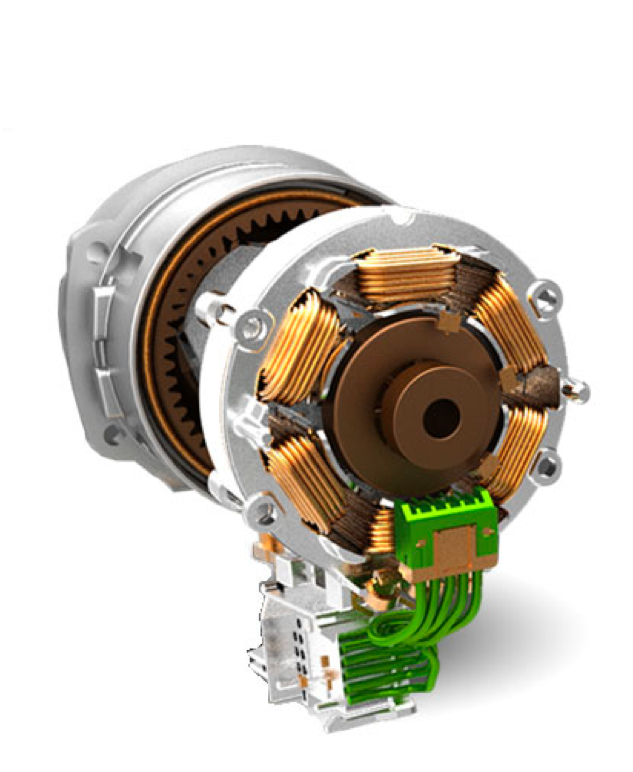
\includegraphics[width=2in]{render.png}
\end{center}
\end{frame}

\begin{frame}{Overview}
\begin{itemize}
  \item {\large Background}\\
  Brushless DC Motors
  \item {\large Theory}\\
  Magneto-statics, Permanent Magnets, Non Linear FEM
  \item {\large Implementation}\\
  Meshing, Matrix Assembly, Solving, Newton Raphson
  \item {\large Results}\\
  Diagrams, Torques
\end{itemize}

\end{frame}
\begin{frame}{Implementation: FEA\textit{lite}}
\hspace{-0.72cm}

\includegraphics[width=4.5in]{technology.pdf}

\end{frame}

\begin{frame}{Implementation: Mesh Generation}
\begin{itemize}
    \item Meshes are generated using the Mathematica 12 mesh generator
    \item Exported as:\\ list of coordinates [$x$, $y$]$^v$ \\list of mesh elements [$v_1$, $v_2$, $v_3$, marker]$^{e}$ \\list of boundary elements [$v_1$, $v_2$, marker]$^{be}$
\end{itemize}


\begin{figure}
    \centering
    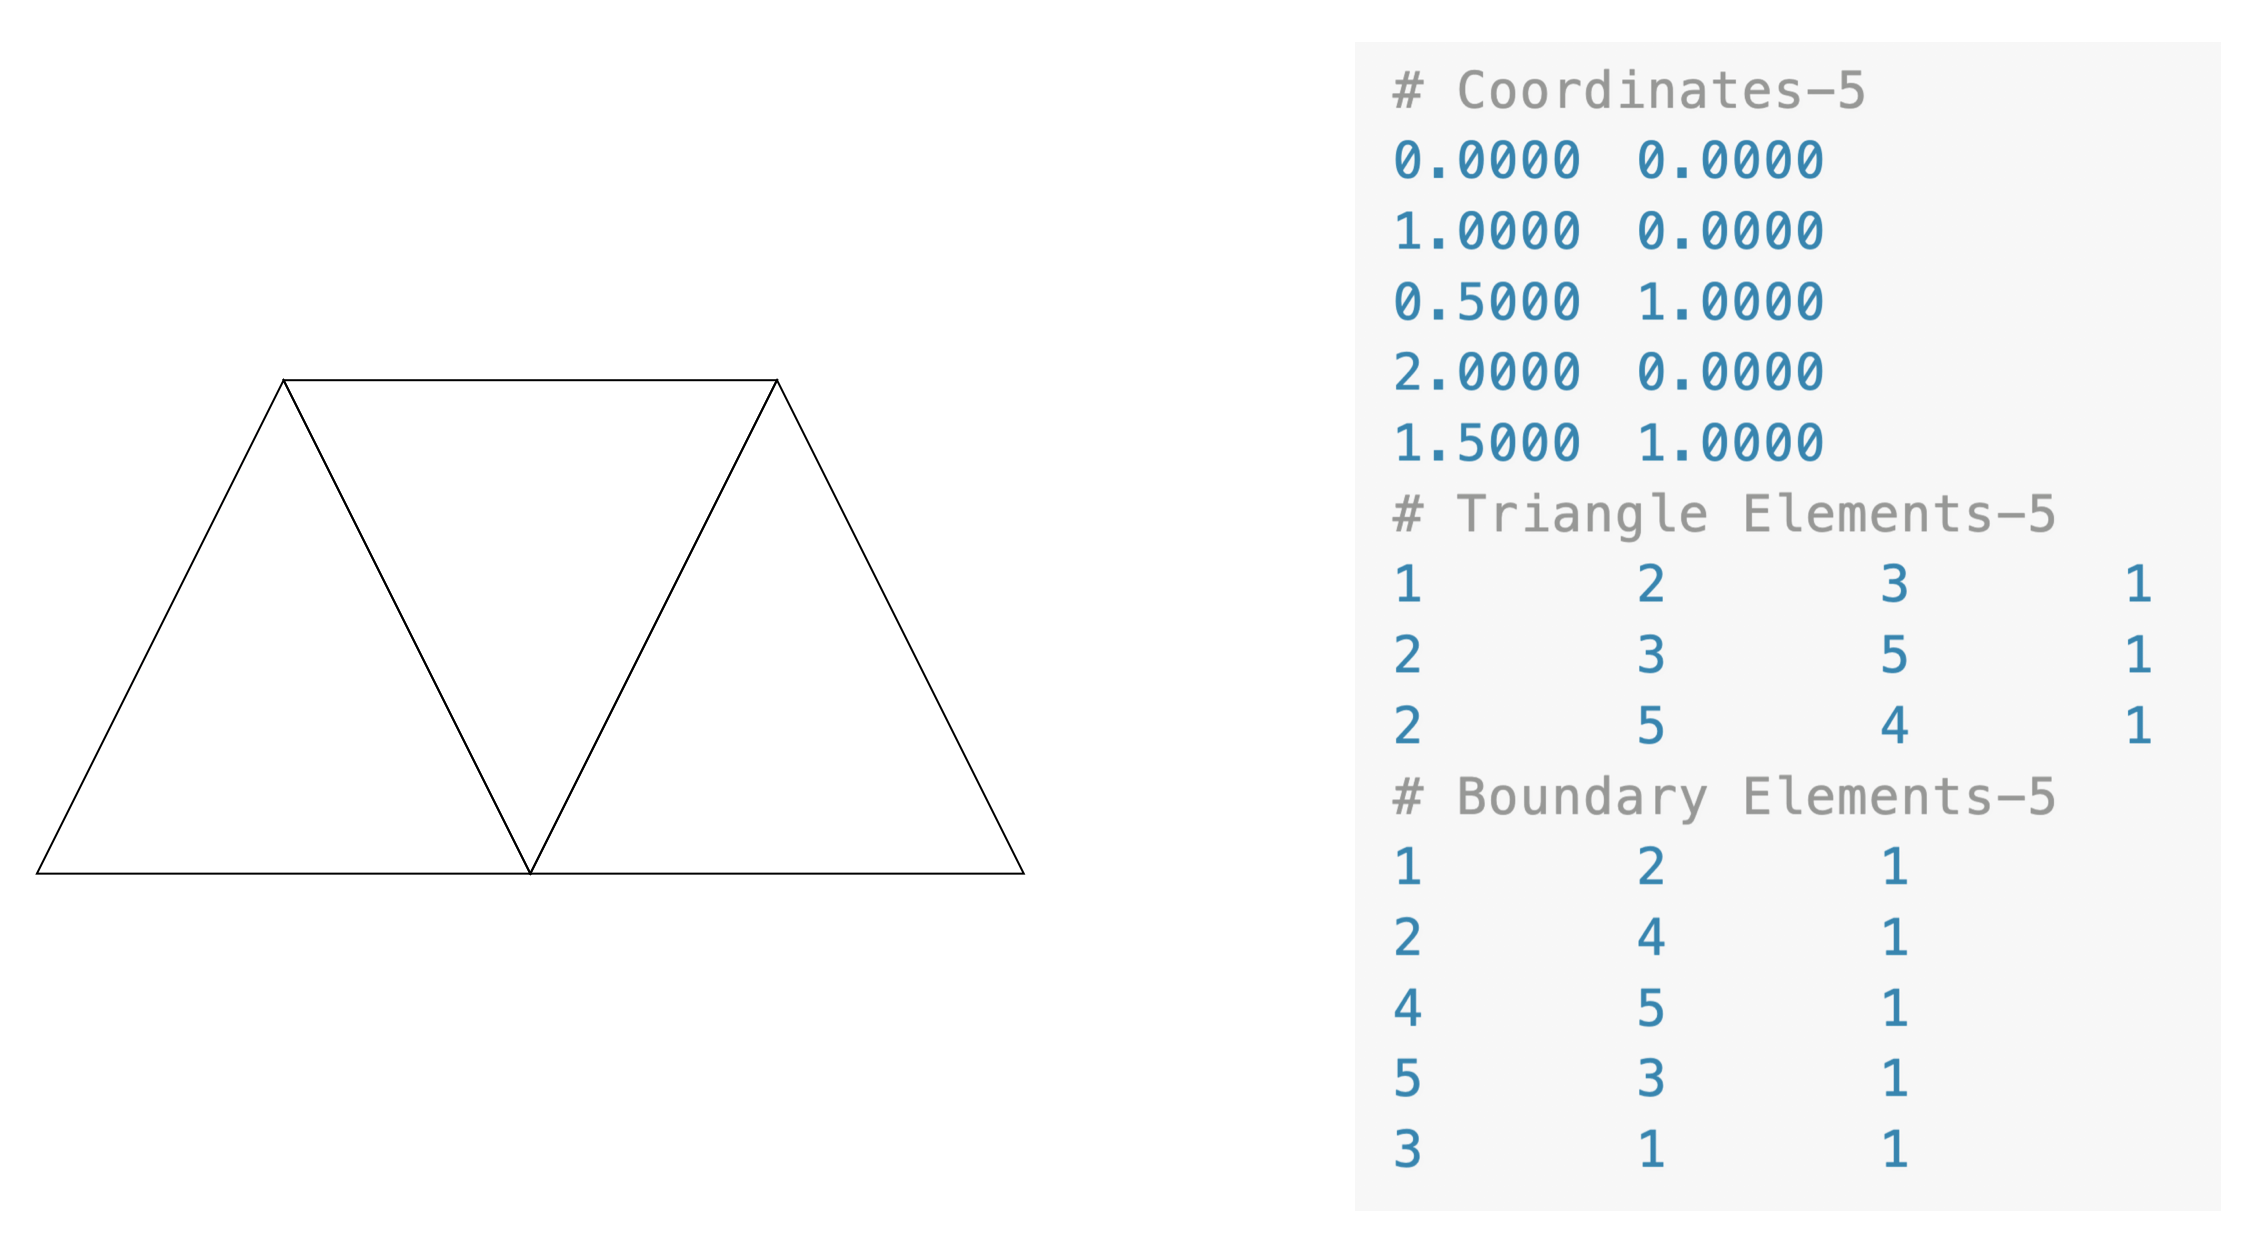
\includegraphics[width=3.5in]{meshdemo.png}
\end{figure}
    
\end{frame}
\begin{frame}{Implementation: Mesh}
    \begin{itemize}
        \item
    \end{itemize}
\end{frame}
\end{document}
